% sample.tex v1.0
% Last Update: 2023-07-14
% Author: 송다은 Daeun Song, daeun7250@gmail.com
% 
% SNU template을 기반으로 이화여자대학교 논문 규격에 맞춰 수정하였습니다.
% 개인적으로 사용하려고 작성하였기 때문에 오류가 있을 수 있습니다.
%
% 한글폰트 휴먼명조체(HMFMM.ttf)는 저작권 상의 이유로 프로젝트에 직접 포함되어 있지 않습니다.
% 폰트를 다운받아 해당 프로젝트에 동일한 이름으로 함께 업로드 하면 문제없이 컴파일 됩니다.
%
% ewhacse.cls file을 사용합니다.
% 박사의 경우 \documentclass[doctor]{ewhacse} (default)
% 석사의 경우 \documentclass[master]{ewhacse} 로 변경하면 됩니다.
% ewhacse.cls file명이 바뀔경우에는 {ewhacse} 대신에 {바뀐 file명}을 넣으면 됩니다.
% 주어진 .cls file의 내용을 변경하는 것은 규격에 어긋난 결과를 낼 수 있습니다.
%
% 주어진 .cls file은 이화여자대학교 논문 규격에 맞춰서 작성되어 있으며,
% MS Word 양식과 동일한 output을 내도록 작성되어 있으므로
% 특별한 설명이 없는 부분은 Word양식의 guideline을 참조하시면 됩니다.
\documentclass[doctor]{ewhacse}

%
% 논문 작성을 위한 사전 준비과정
% 논문제목 (국문, 영문), 저자, 제출일, 심사일, 졸업일의 정보를 넣습니다.

% 논문제목을 넣습니다.
% 필히 한글제목과 영문제목 모두 넣어야 합니다.
\title[korean]{논 문 제 목}
\title[english]{Predictive Habitat Model for Eurasian Otter (Lutra lutra) inhabiting in the catchment of Naechon and Kuneob river}

% 저자 정보를 넣습니다.
% 국문성명, 영문성명 모두 넣어야 하며, 특히 국문성명의 경우는 글자사이에 space가 있는 것과 없는 것
% 두 가지 모두를 집어넣어줘야 합니다.
\author[korean]{송 다 은}
\author[english]{Daeun Song}
\author[nospace]{송다은}
% 소속
\department[korean]{인공지능·소프트웨어학부}
\department[space]{인 공 지 능  ·  소 프 트 웨 어 학 부}
\school{이화여자대학교 대학원} 

% 지도교수님의 성함을 국문으로 넣습니다.
\adviser{김 영 준}

% 심사위원 교수님들의 성함을 국문으로 넣습니다. (석사과정 3인, 박사과정 5인)
\commitee[1]{오 유 란}
\commitee[2]{류 석 창}
\commitee[3]{윤 성 의}
\commitee[4]{이 주 행}
\commitee[5]{김 영 준}

% 논문 제출일, 논문 심사일을 한글로 넣습니다.
\submissiondeadline{20022 년 ~~ 12 월} \examinationdate{20022 년 ~~ 12 월}
\examinationyear{2022}

% 졸업일을 영문식, 한글식 두 가지 방법 모두 넣습니다.
\gradyear[english]{2023} \gradyear[korean]{2023}

%

% 문서의 시작
%
% 위의 정보들을 빠짐없이 채워넣고 document를 시작하면
% 외표지, 내표지(외표지와 동일), 인준지가 자동으로 생성됩니다.

% 문단 indentation 크기
\setlength{\parindent}{1em}
\setlength{\parskip}{1em}

\begin{document}
\renewcommand{\baselinestretch}{1.8}    % 본문의 줄간격 조정, 고치거나 삭제하지 마십시오.
\fontsize {10.5pt}{10.5pt}
\selectfont 

%\changepage{5mm}{}{}{}{}{}{}{}{-5mm}    %%페이지 여백 재설정. 절대 고치거나 삭제하지 마십시오.
\makelists   %목차를 자동생성합니다.

% abstract(영문)의 작성
% begin과 end 사이에 abstract의 내용을 채워넣습니다.
\begin{abstract}
\par %abstract 첫 문장 들여쓰기, 고치거나 삭제하지 마십시오.
This tex file gives you guidelines for preparing the thesis for Ewha Womans University. 
This document can be used as a template for the thesis. 
You can easily make your thesis document using this template. You can freely put your chapters,
sections in this tex file.
Do not change ewhacse.cls file and do not remove specified
command lines in this sample file.

Title and other information in abstract like name and affiliation can be
omitted. Keywords and student number should be located at bottom of
page. We hope this document be helpful to writing a thesis. English character font type is	Times New Roman, Korean character font type is HumanMyoungJo(휴먼명조체).

Please refer to the university-provided guideline for specific details, such as line spacing, paper margin, etc. 
	
\end{abstract}

% 본문의 시작
% chapter, section의 추가,변경등 모두를 자유롭게 할 수 있습니다.
% 그림, 표의 추가 형식은 MS Word의 형식과 동일합니다. (MS Word Description file 참조)
%
\chapter{Introduction}
\par %abstract 첫 문장 들여쓰기, 고치거나 삭제하지 마십시오.

\section{Study object}
\lipsum[1]

\chapter{Chapter Example}

\section{Section Example}
\par %abstract 첫 문장 들여쓰기, 고치거나 삭제하지 마십시오.

\lipsum[1]

\subsection{Subsection Example}

\lipsum[1]

\lipsum[1]

\subsection{Subsection Example}

\lipsum[1]

\section{Section Example}

\lipsum[1]

\chapter{Figures and Tables}
\section{Figures}
\par %abstract 첫 문장 들여쓰기, 고치거나 삭제하지 마십시오.

\lipsum[1]

\begin{figure}[htbp]
	{
		\begin{center}
			\begin{tabular}{c}
				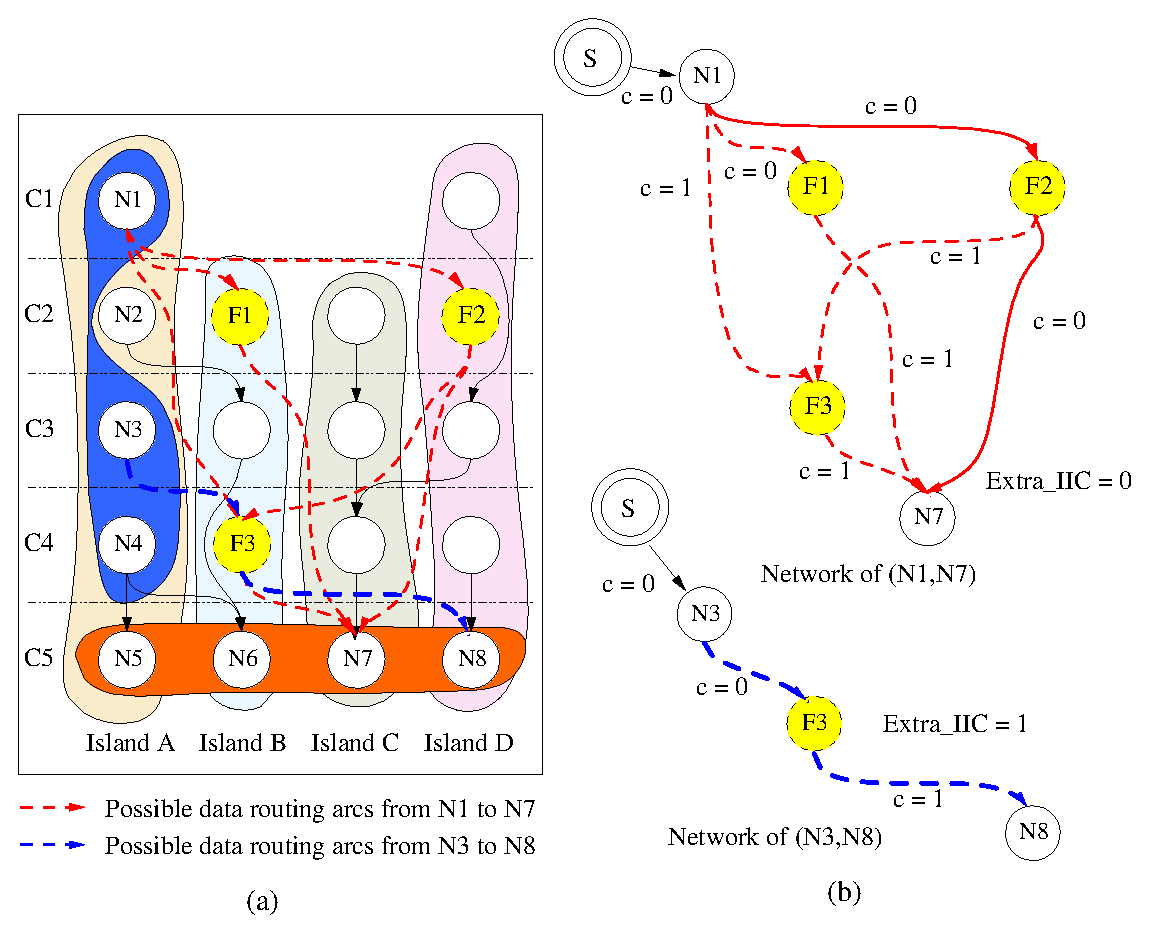
\includegraphics[height=6cm]{Sample.eps}
			\end{tabular}
		\end{center}
	}
	\caption{Example 1}
\end{figure}

\newpage
If the caption of the figure is longer than one lines, you should align it left.(This is default)\\

\begin{figure}[htbp]
	{
		\begin{center}
			\begin{tabular}{c}
				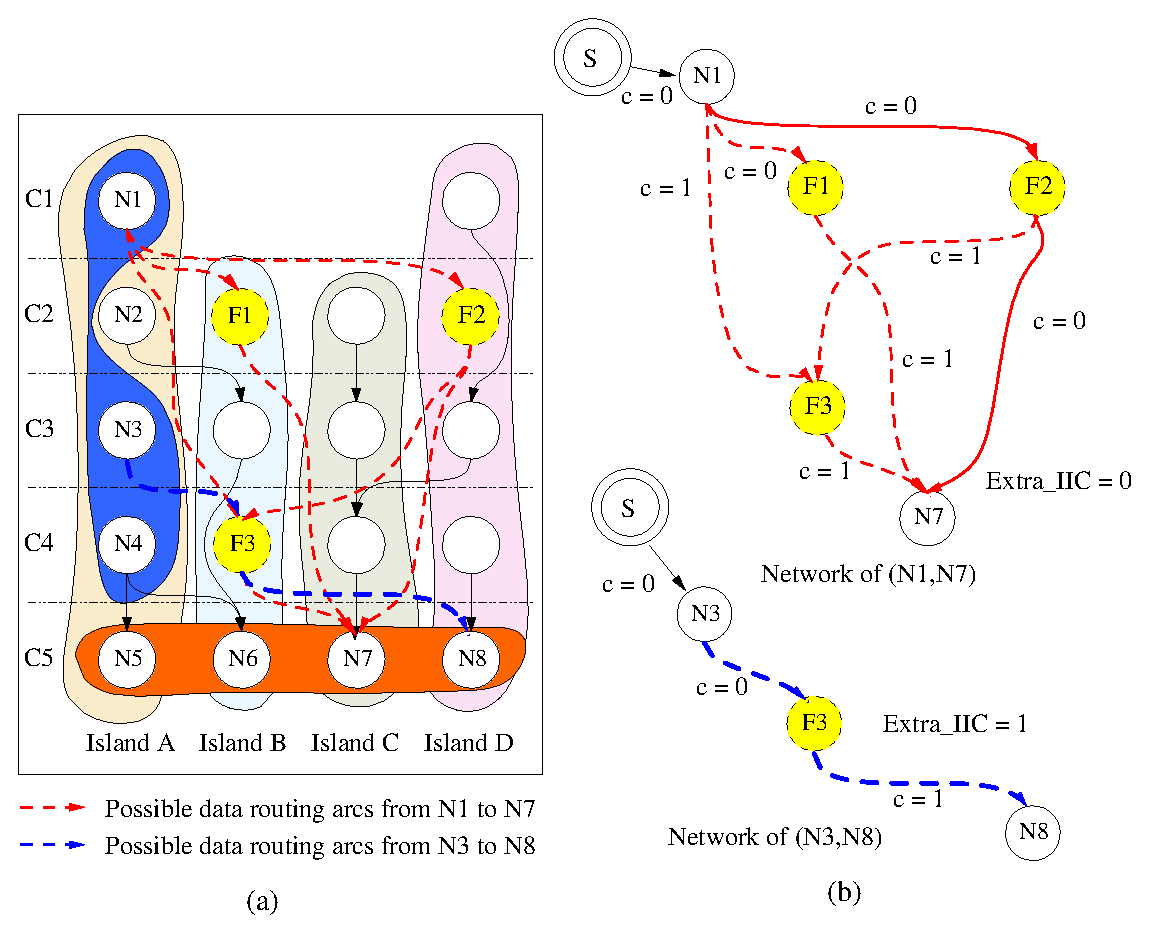
\includegraphics[height=6cm]{Sample.eps}
			\end{tabular}
		\end{center}
	}
	\caption{itam, que ipiti sum dem velit la sum et dionet quatibus apitet voloritet audam, qui aliciant voloreicid quaspe volorem ut maximusandit faccum conemporerum aut ellatur}
\end{figure}
\newpage

\section{Tables}
\par %abstract 첫 문장 들여쓰기, 고치거나 삭제하지 마십시오.

This is example of inserting your tables in your thesis. The
caption of the table should be located above the table. Be
careful that caption should not end with '.'
\begin{table}[htbp]
	\begin{center}
		\caption{Example 3} \label{tab1}
		\begin{tabular}{|c|c|c|} \hline
			Benchmarks & Number of nodes  & L\\ \hline
			\hline {\sc chen} & 87  & 14\\ \hline {\sc 3d\_force1} & 53  & 15\\
			\hline {\sc 3d\_force2} & 36  & 11\\ \hline {\sc 3d\_motion} & 45  &
			6\\ \hline {\sc mpeg\_calcid} & 27  & 8\\ \hline {\sc adpcm\_dec} &
			15  & 6 \\ \hline {\sc jm\_itrans} & 58  & 9\\ \hline {\sc 4ar} & 28
			& 8\\ \hline
		\end{tabular}
	\end{center}
\end{table}


\chapter{New Chapter}

\lipsum[1]

%
% 참고문헌을 넣습니다.
% 샘플의 형식과 같은 차례대로 써줍니다.
%
% bibtex 사용 가능
% bibtex 사용 예시:
% \bibliographystyle{IEEEtran}{}
% \addcontentsline{toc}{chapter}{Bibliography}
% \bibliography{sample} 

\begin{thebibliography}{00}
    \addcontentsline{toc}{chapter}{Bibliography}
	
	% 영문저널의 경우
	\bibitem{ref1} B. Jeon and J. Jeong, ``Blocking artifacts
	reduction in image compression with block boundary discontiunity
	criterion,'' {\em IEEE Transactions on Circuits and Systems for
		Video Tech.}, vol. 8, no.3, pp. 345-357, June 1998.
	
	% 영문학술대회의 경우
	\bibitem{ref2} W. G. Jeon and Y. S. Cho, ``An equalization
	technique for OFDM and MC-CDMA in a multipath fading channels,''
	in {\em Proceedings of IEEE Conference on Acoustics, Speech and
		Signal Processing}, Munich, Germany, May 1997. pp. 2529-2532.
	
	% 국내저널의 경우
	\bibitem{ref3} 김남훈, 정영철, ``평탄한 통과대역 특성을 갖는
	새로운 구조의 광도 파로열 격자 라우터,'' {\em 전자공학회논문지},
	제35권 D편, 제3호, 56-62쪽, 1998년 3월.
	
	% 국내학술대회의 경우
	\bibitem{ref4} 윤남국, 김수종, ``무선 센서 네트워크에서의 에너지
	효율적인 그라디언트 기반 라우팅 기법,'' {\em 한국정보과학회
		2006년 추계학술대회}, 제12권, 제2호, 2006년 10월. pp.
	1372-1374.
	
	% 단행본의 경우
	\bibitem{ref5} C. Mead and L. Conway, {\em Introduction to VLSI
		Systems}, Addison-Wesley, Boston, 1994.
	
	% URL
	\bibitem{ref6} The SolarMESH Network,
	http://owl.mcmater.ca/solarmesh
	
	% Technical Report의 경우
	\bibitem{ref7} K. E. Elliott and C. M. Greene, ``A local adaptive
	protocol,'' Argonne National Laboratory, Argonne, France,
	Technical Report 916-1010-BB, 1997.
	
	% 학위논문의 경우
	\bibitem{ref8} T. Kim, ``Scheduling and Allocation Problems in
	High-level Synthesis,'' Ph. D. Dissertation, ECE Department,
	Univ. of Illinois at U-C, 1993.
	
	% 특허의 경우
	\bibitem{ref9} Sunghyun Choi, ``Wireless MAC protocol based on a
	hybrid combination of slot allocation, token passing, and
	polling for isochronous traffic,'' U.S. Patent No. 6,795,418,
	September 21, 2004.
	
	% 표준
	\bibitem{ref10} IEEE Std. 802.11-1999, Part 11: Wireless LAN
	Medium Access Control (MAC) and Physical Layer (PHY)
	specifications, Reference number ISO/IEC 8802-11:1999(E), IEEE
	Std. 802.11, 1999 edition, 1999.

	
\end{thebibliography}

%---------------------------------------------------------------------------------
% 본문의 종료
% 국문 초록과 감사의 글(선택)을 넣습니다.
% begin{summary}와 end{summary}의 사이에 국문초록을 집어넣습니다.
% 감사의글은 \acknowledgement{}의 대괄호 안에 내용을 넣습니다.
%
\begin{summary}
    \fontsize {10.5pt}{10.5pt}
    \selectfont 
	\par    %첫 줄 들여쓰기를 위한 단락구분.삭제하지 마십시오.
	최근 시민사회에 대한 높은 관심과 활발한 논의에도 불구하고, 1990년대 이후의 동아시아의 시민사회에 대한 연구는 충분히 이루어지지 못하고 있다. 또한, 기존의 연구들은 대부분 동아시아 시민사회의 전반적인 발전양상에 대해서만 다룰 뿐, 동아시아
\end{summary}
%\changepage {15mm}{}{}{}{}{-30mm}{}{}{15mm} %초록과 감사의 글을 위한 여백 재설정, 고치거나 삭제하지 마십시오.
\acknowledgement{
	\par
	감사의 글

 %감사의 글을 작성하지 않을경우 삭제가능
}

\end{document}
